\section{Self-evolving Agentic Reasoning}
\label{sec:selfevolve}

Self-evolving agentic reasoning refers to an agent’s capacity to \emph{improve its own reasoning process through experience}. 
At the core of this evolution lie two fundamental mechanisms: \textbf{feedback} and \textbf{memory}. 
\textbf{Feedback} provides evaluative signals for self-correction and refinement, allowing the agent to revise its reasoning strategies based on outcomes or environmental responses. 
\textbf{Memory}, in turn, acts as a persistent substrate for storing, organizing, and synthesizing past interactions, enabling knowledge accumulation and reuse across tasks. 
Together, these mechanisms transform reasoning from a static process into a dynamic, adaptive loop capable of continual improvement.

Building upon foundational capabilities such as \emph{planning}, \emph{search}, and \emph{tool use}, self-evolving agents integrate feedback and memory to refine their internal reasoning policies, adjust decision-making strategies, and generalize across diverse contexts, often without explicit external supervision. 
This continual adaptation marks a critical step toward lifelong reasoning and lays the groundwork for the collective intelligence explored in the next section.






\subsection{Agentic Feedback Mechanisms}

Agentic feedback mechanisms enable models to iteratively refine their reasoning and actions rather than relying on one-shot responses. By incorporating self-critique, verifier guidance, or validator-based resampling, these methods emulate human trial-and-error learning and form the foundation for autonomous self-improvement. Broadly, they operate through three distinct feedback regimes:
(1) reflective feedback, where models revise their reasoning through self-critique or verification;
(2) parametric adaptation, where feedback is consolidated into updated model parameters; and
(3) validator-driven feedback, where binary outcome signals guide resampling without introspection.

These regimes define a continuum between dynamic, inference-time adaptability, durable learning through parameter updates, and efficient correction through external signals. Together, they highlight how modern agents leverage feedback to balance flexibility, reliability, and efficiency.

\subsubsection{Reflective Feedback}

Reflective feedback methods improve model reliability by modifying the reasoning process during inference, without updating model parameters. These approaches expose intermediate reasoning outputs, such as chains of thought or partial solutions, and introduce additional assessment steps that directly influence how the model continues its generation.

Early self-critique and rationale-refinement methods \cite{shinn2023reflexion,madaan2023self} implement reflection through an explicit generate–critique–revise loop. A model first produces an answer together with its reasoning. The same model, or a separately prompted critic role, then analyzes this output to identify logical errors, unsupported assumptions, or missing steps. The critique is appended as context for a revised generation, and this process may be repeated multiple times or augmented with external evidence such as retrieval. More recent self-improvement frameworks \cite{selfimprovement2024a} extend reflective feedback beyond a single inference episode by accumulating critiques or failure cases across interactions. Instead of correcting only one response, these methods reuse past feedback to guide future generations through prompt refinement or curated supervision signals, while still operating without direct parameter updates at inference time. Search-based reasoning strategies \cite{wangself,yao2023tree,besta2024graph} improve reliability by generating and comparing multiple candidate reasoning paths. These methods explore the solution space through stochastic sampling or structured search, then select or aggregate outputs using voting schemes, heuristic scores, or learned evaluators. Improvement arises from comparison across alternatives rather than explicit revision of a single reasoning trajectory. Decomposition-based prompting methods \cite{zhou2022least,chenprogram} reformulate complex problems into ordered sequences of simpler subproblems. Intermediate results are reused in later steps, allowing partial inspection of reasoning progress and reducing error propagation, even when no explicit critique step is introduced.

Overall, reflective feedback alters inference-time reasoning trajectories by introducing additional reasoning or comparison steps. Feedback is used to guide generation within an episode, while the model’s parameters remain unchanged.

\begin{figure}
    \centering
    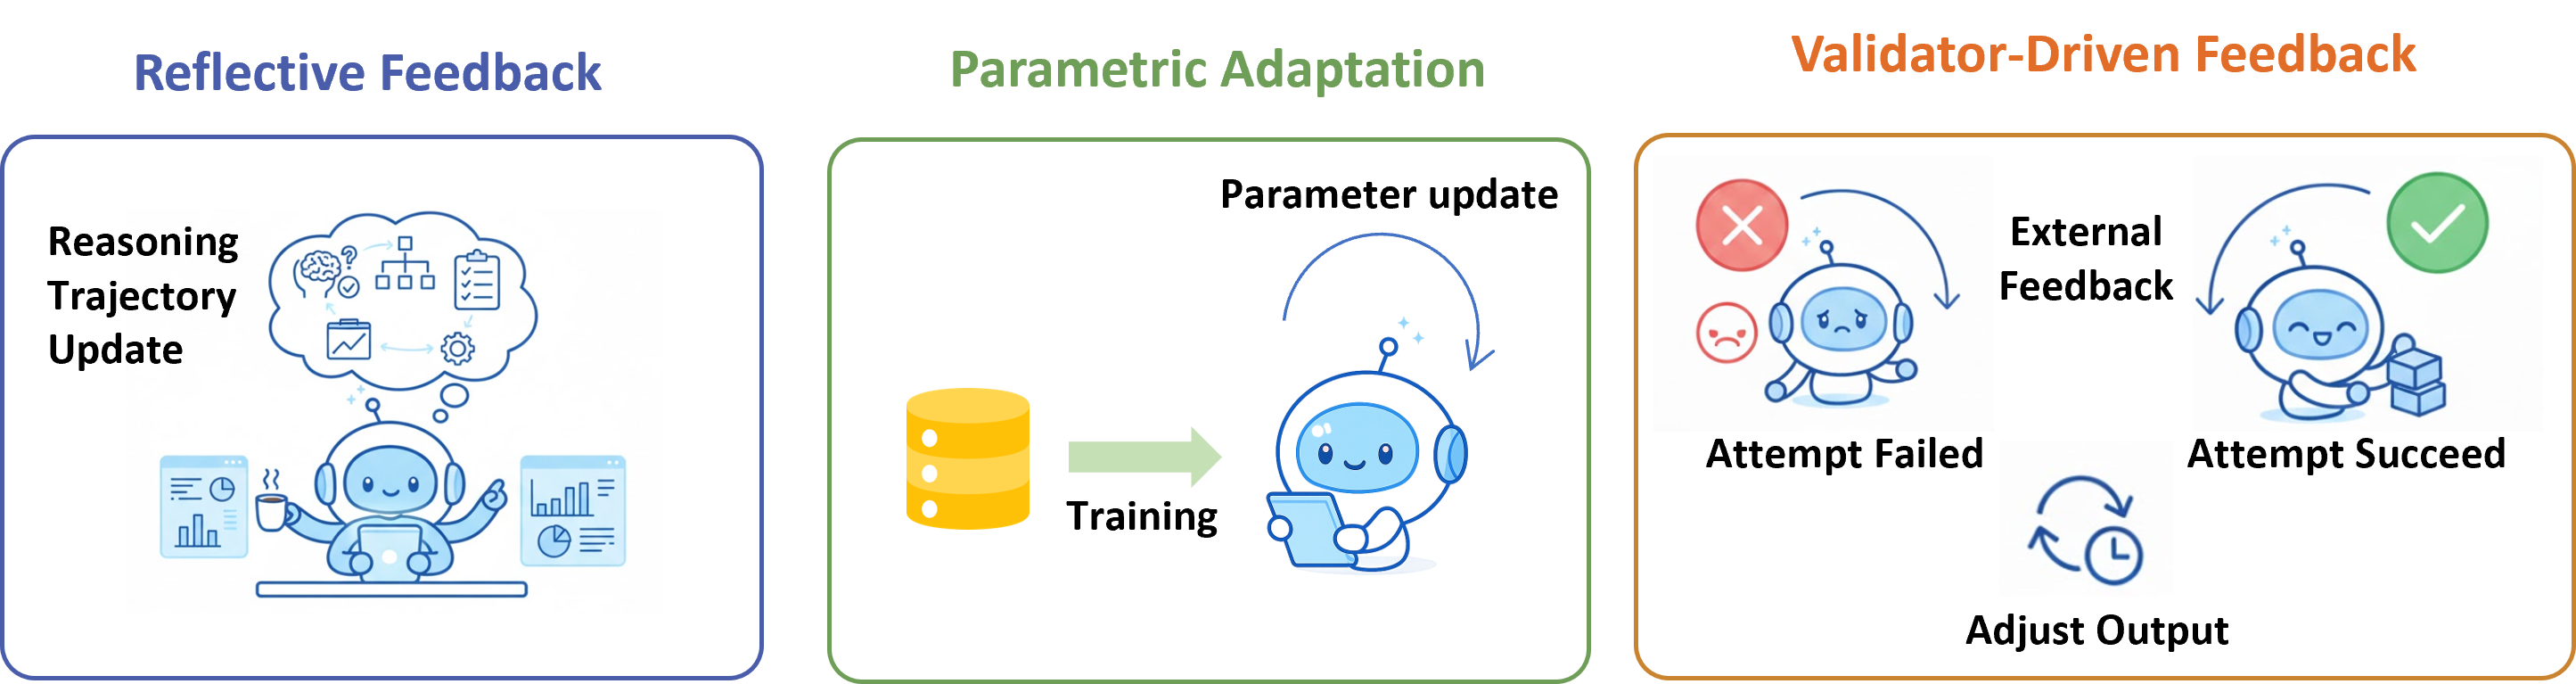
\includegraphics[width=\linewidth]{arxiv/figs/feedback.png}
    \caption{
    \textbf{Illustration of three forms of agentic feedback mechanisms.}
    \textit{Inference-time reflection} enables real-time self-critique and revision during reasoning;
    \textit{offline adaptation} consolidates feedback into model parameters for long-term improvement;
    and \textit{outcome-based feedback} relies on validator signals (success or failure) to refine behavior through retry.
    Together, they represent a continuum from adaptive reflection to stable learning and efficient validation.
    }
    \label{fig:agentic_feedback}
\end{figure}

\subsubsection{Parametric Adaptation}

Parametric adaptation incorporates feedback into a model’s parameters through additional training, producing persistent behavioral changes that generalize beyond individual inference episodes. Unlike reflective feedback, these methods transform feedback signals into supervised or preference-based training objectives that update the model’s weights.

Trajectory-level supervised fine-tuning approaches \cite{zeng2024agenttuning,aksitov2023rest} attach feedback to intermediate reasoning traces rather than only final answers. Models first generate multi-step trajectories, which are then reviewed by humans, auxiliary models, or automated verifiers. Incorrect steps are corrected or replaced, and the resulting feedback-enriched trajectories are used as supervised training data, encouraging the model to internalize improved reasoning patterns. Distillation-based methods \cite{hsieh2023distilling} further leverage improved reasoning traces by training student models on high-quality chains of thought or self-corrected solutions generated by stronger teachers. This process transfers structured reasoning behaviors into more stable or efficient models, removing the need for explicit reflection at inference time. Preference-alignment approaches \cite{christiano2017deep,rafailov2023dpo,bai2022constitutional} incorporate feedback in the form of comparative judgments that distinguish preferred from dispreferred outputs. Training objectives such as reward modeling or direct preference optimization adjust the model’s parameters so that preferred behaviors become more likely. Although feedback is often defined over final outputs, it implicitly shapes the internal reasoning strategies that produce them. Recent work shows that verification-augmented training data can further improve reasoning robustness across domains \cite{li2025reflectevo,zheng2025reasoningcv}. In these settings, trajectories are filtered or revised based on correctness or consistency signals before training, yielding datasets that emphasize reliable reasoning patterns.

In summary, parametric adaptation embeds feedback directly into the model’s parameters, yielding durable improvements across tasks. This durability comes at the cost of additional training and reduced flexibility compared to inference-time methods.

\subsubsection{Validator-Driven Feedback}

Validator-driven feedback improves model outputs using external success or failure signals, without modifying the model’s reasoning process or parameters. A validator, such as a unit test, constraint checker, simulator, or environment signal, evaluates candidate outputs and determines whether they satisfy predefined correctness criteria.

Retry-based systems \cite{dao2025rezero,potamitis2025retrials} implement this paradigm by repeatedly sampling candidate outputs until one passes validation. The model generates a complete solution, submits it to the validator, and discards it if validation fails. Subsequent attempts are generated independently, without conditioning on explicit information about previous failures. This strategy is particularly effective in domains with reliable and inexpensive validation, such as program synthesis and software engineering \cite{le2022coderl,ni2023lever,swebench}. Generated code can be executed against unit tests, providing an unambiguous correctness signal. The model iterates until a solution satisfies all tests, even in the absence of explicit reasoning correction. Similar mechanisms appear in embodied and interactive agents \cite{ahn2022icanisay,driess2023palm}, where action sequences are repeatedly executed until the environment signals task completion. Failed sequences are abandoned and new ones are attempted, based solely on external success signals. Some hybrid methods introduce lightweight guidance within the retry loop, for example by assigning higher reward to behaviors that eventually lead to successful outcomes \cite{bensal2025reflect}. However, the dominant mechanism remains selection through external validation rather than revision of reasoning steps or parameter updates.

Overall, validator-driven feedback offers an efficient and scalable way to improve output correctness when reliable validators are available. Its limitation is that feedback is non-diagnostic, correcting individual outputs without explaining failures or altering the model’s reasoning behavior.

\begin{table*}[!t]
\centering
\caption{Representative \textbf{Agentic Feedback Mechanisms} categorized by \textit{Feedback Stage}, \textit{Feedback Source}, and \textit{Update Target}.}
\renewcommand{\arraystretch}{1.15}
\setlength{\tabcolsep}{3pt}
\begin{tabular}{p{5.5cm}
  >{\centering\arraybackslash}p{3.8cm}
  >{\centering\arraybackslash}p{4.8cm}
  >{\centering\arraybackslash}p{3.3cm}}
\toprule
\textbf{Method / System} & \textbf{Feedback Stage} & \textbf{Feedback Source} & \textbf{Update Target} \\
\midrule

%%%%%%%%%%%%%%%%%%%%%%%%%%%%%%%%%%%%%%%%%%%%%%%%%%%%%%%%%%%%%%
% I. Reflective Feedback
%%%%%%%%%%%%%%%%%%%%%%%%%%%%%%%%%%%%%%%%%%%%%%%%%%%%%%%%%%%%%%
\rowcolor[HTML]{F5F5F5}
\multicolumn{4}{l}{\textbf{I. Reflective Feedback}} \\

Reflexion~\cite{shinn2023reflexion} & Inference & Self-generated critique & Trajectory \\
Self-Refine~\cite{madaan2023self} & Inference & Self-evaluation & Trajectory \\
Constitutional AI~\cite{bai2022constitutional} & Inference & Normative rules & Trajectory \\
RLAIF~\cite{lee2023rlaif} & Inference & AI verifier & Trajectory \\
SelfCheckGPT~\cite{manakul2023selfcheckgpt} & Inference & Cross-sample divergence & Trajectory \\
Zero-Shot Verification-CoT~\cite{chowdhury2025zeroshot} & Inference & External verifier & Trajectory \\
ASCoT~\cite{zhang2025ascot} & Inference & Vulnerability detection & Trajectory \\
MM-Verify~\cite{sun2025mmverify} & Inference & Multimodal verifier & Trajectory \\
ReAct~\cite{yao2023react} & Inference & Action outcomes & Trajectory \\
PAL~\cite{gao2023pal} & Inference & Code execution & Trajectory \\
WebGPT~\cite{nakano2021webgpt} & Inference & Web evidence & Trajectory \\
MemGPT~\cite{Packer2023MemGPTTL} & Inference & Retrieved memory & Trajectory \\
Voyager~\cite{wang2023voyager} & Inference & Environment + memory & Trajectory \\

\midrule

%%%%%%%%%%%%%%%%%%%%%%%%%%%%%%%%%%%%%%%%%%%%%%%%%%%%%%%%%%%%%%
% II. Parametric Adaptation
%%%%%%%%%%%%%%%%%%%%%%%%%%%%%%%%%%%%%%%%%%%%%%%%%%%%%%%%%%%%%%
\rowcolor[HTML]{F5F5F5}
\multicolumn{4}{l}{\textbf{II. Parametric Adaptation}} \\

AgentTuning~\cite{zeng2024agenttuning} & Training & High-quality trajectories & Model parameters \\
ReST~\cite{aksitov2023rest} & Training & Critique--revision pairs & Model parameters \\
ReFT~\cite{dou2024re} & Training & Reflection-augmented data & Model parameters \\
Distill-CoT~\cite{hsieh2023distilling} & Training & Expert CoT & Model parameters \\
ReflectEvo~\cite{li2025reflectevo} & Training & Reflection traces & Model parameters \\
Reasoning-CV~\cite{zheng2025reasoningcv} & Training & Verification signals & Model parameters \\

\midrule

%%%%%%%%%%%%%%%%%%%%%%%%%%%%%%%%%%%%%%%%%%%%%%%%%%%%%%%%%%%%%%
% III. Validator-Driven Feedback
%%%%%%%%%%%%%%%%%%%%%%%%%%%%%%%%%%%%%%%%%%%%%%%%%%%%%%%%%%%%%%
\rowcolor[HTML]{F5F5F5}
\multicolumn{4}{l}{\textbf{III. Validator-Driven Feedback}} \\

ReZero~\cite{dao2025rezero} & Inference & Binary validator & Output only \\
Retrials~\cite{potamitis2025retrials} & Inference & Acceptance signal & Output only \\
CodeRL~\cite{le2022coderl} & Inference & Unit tests & Output only \\
LEVER~\cite{ni2023lever} & Inference & Execution results & Output only \\
SWE-bench~\cite{swebench} & Inference & Test suite & Output only \\
SayCan~\cite{ahn2022icanisay} & Inference & Environment state & Output only \\
PaLM-E~\cite{driess2023palm} & Inference & Environment feedback & Output only \\
Reflect--Retry--Reward~\cite{bensal2025reflect} & Inference & Validator + reflection signal & Output only \\

\bottomrule
\end{tabular}
\label{tab:agentic_feedback_methods}
\end{table*}






\subsection{Agentic Memory}

Recent advances in memory-augmented LLM agents have shifted the focus from static memory storage to more dynamic, interactive mechanisms that directly support agentic reasoning. Rather than merely extending the context window or storing historical inputs, memory is increasingly treated as an integral component of the reasoning loop, used for reflecting on past experiences, guiding future actions, and dynamically adapting to complex, long-horizon tasks. Formally, an agent maintains a memory module where each memory entry may represent a raw observation, summarized trajectory, subgoal, tool invocation trace, or other structured element depending on the system design.


The agent’s reasoning process then operates not only on its immediate context but also on this persistent memory, enabling reflection, generalization, and long-term goal tracking. In this section, we organize prior work along four emerging trends in the use of memory to support and enable agentic reasoning. Figure \ref{fig:agentic_memory} summarizes how agentic memory progresses from contextual recall to adaptive control.
In-context memory captures textual and semantic information from prior interactions; structured memory integrates these into graph and multimodal representations; post-training control enables agents to evolve, update, and retrieve memory through learned reward-based mechanisms.

\begin{figure}
    \centering
    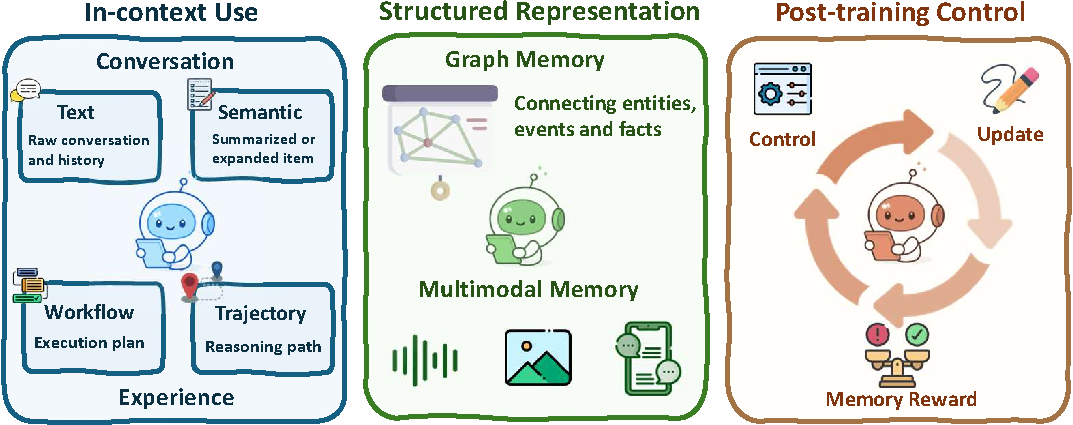
\includegraphics[width=\linewidth]{arxiv/figs/memory.pdf}
    \caption{Overview of \textbf{Agentic Memory} in LLM agents, showing three parallel dimensions:
in-context use (text and experience), structured representation (graph and multimodal memory), and post-training control (reward-guided memory management).}
    \label{fig:agentic_memory}
\end{figure}


\begin{table*}[!t]
\centering
\caption{Representative \textbf{Agentic Memory} systems categorized by \textit{Setting}, \textit{Format}, and \textit{Memory Type}.}
\renewcommand{\arraystretch}{1.15}
\setlength{\tabcolsep}{6pt}
\begin{tabular}{p{5cm}>{\centering\arraybackslash}p{3.0cm}
  >{\centering\arraybackslash}p{3.0cm}
  >{\centering\arraybackslash}p{3.0cm}}
\toprule
\textbf{Method / System} & \textbf{Setting} & \textbf{Format} & \textbf{Memory Type} \\
\midrule

\rowcolor[HTML]{F5F5F5}
\multicolumn{4}{l}{\textbf{I. Agentic Use of Flat Memory (In-Context)}} \\

LangMem~\cite{LangChain2023} & In-Context & Text & Factual \\
LlamaIndex~\cite{Liu_LlamaIndex_2022} & In-Context & Text & Factual \\
MemGPT~\cite{Packer2023MemGPTTL} & In-Context & Text & Factual \\
MemoryBank~\cite{Zhong2023MemoryBankEL} & In-Context & Semantic & Factual \\
Amem~\cite{xu2025mem} & In-Context & Semantic & Factual \\
Workflow Memory~\cite{Wang2024AgentWM} & In-Context & Workflow & Experience \\
MemOS~\cite{li2025memos} & In-Context & Semantic & Factual \\
LightMem~\cite{fang2025lightmem} & In-Context & Semantic & Factual \\
Nemori~\cite{nan2025nemori} & In-Context & Semantic & Factual \\
ACE~\cite{zhang2025agentic} & In-Context & Workflow & Experience \\
Reasoning Bank~\cite{ouyang2025reasoningbank} & In-Context & Workflow & Experience \\
Dynamic Cheatsheet~\cite{suzgun2025dynamic} & In-Context & Trajectory & Experience \\
Sleep-time Compute~\cite{Lin2025SleeptimeCB} & In-Context & Trajectory & Experience \\
Evo-Memory~\cite{wei2025evo} & In-Context & Semantic & Experience \\
\midrule
\rowcolor[HTML]{F5F5F5}
\multicolumn{4}{l}{\textbf{II. Structured Memory Representations}} \\

GraphRAG~\cite{Edge2024FromLT} & In-Context & Graph & Factual \\
MEM0~\cite{chhikara2025mem0} & In-Context & Graph & Factual \\
Zep~\cite{rasmussen2025zep} & In-Context & Graph & Factual \\
Optimus-1~\cite{li2024optimus1} & In-Context & Multimodal & Experience \\
RAP~\cite{rap} & In-Context & Multimodal & Experience \\
M3-Agent~\cite{long2025seeing} & In-Context & Multimodal & Factual \\
Mem-Gallery~\cite{bei2026mem} & In-Context & Multimodal & Factual \\
Agent-ScanKit~\cite{cheng2025agent} & In-Context & Multimodal & Experience \\
% AutoFlow~\cite{Li2024AutoFlowAW} & In-Context & Workflow & Experience \\
% AFLOW~\cite{zhang2024aflow} & In-Context & Workflow & Experience \\
% FlowMind~\cite{Zeng2023FlowMindAW} & In-Context & Workflow & Experience \\

\midrule
\rowcolor[HTML]{F5F5F5}
\multicolumn{4}{l}{\textbf{III. Post-training Memory Control}} \\
Mem1~\cite{zhou2025mem1} & Post-training & Semantic & Factual \\
Memory-as-Action~\cite{zhang2025memory} & Post-training & Semantic & Factual \\
MemAgent~\cite{yu2025memagent} & Post-training & Semantic & Factual \\
Mem-$\alpha$~\cite{wang2025mem1} & Post-training & Semantic & Factual \\
Memory-R1~\cite{yan2025memoryr1} & Post-training & Semantic & Factual \\
Agent Early Experience~\cite{zhang2025agent2} & Post-training & Implicit & Experience \\
Agentic Memory~\cite{yu2026agentic} & Post-training & Semantic & Experience \\
MemRL~\cite{zhang2026memrl} & Post-training & Semantic & Experience \\
\bottomrule
\end{tabular}
\label{tab:agentic_memory_methods}
\end{table*}




\subsubsection{Agentic Use of Flat Memory}


\paragraph{Factual Memory.} Traditional memory systems for LLM agents typically treat memory as a passive buffer, mainly used to store dialogue histories or recent observations to address the limited context window of transformer models. Examples include dense retrieval methods~\cite{lewis2020retrieval,asaiself,Zhong2023MemoryBankEL}, pre-defined modules in LangChain and LLamaIndex~\cite{Liu_LlamaIndex_2022}, and cache-inspired designs like MemGPT~\cite{Packer2023MemGPTTL}. These approaches usually retrieve semantically similar past content to augment prompts, without influencing the agent’s internal reasoning. Enhancements such as RET-LLM with differentiable memory~\cite{Modarressi2023RETLLMTA}, SCM with controller-based mechanisms~\cite{Liang2023SCMEL}, as well as LOCOMO and LongMemEval benchmarks for long-term retention~\cite{maharana2024evaluating,wu2024longmemeval} further improve recall but remain largely static. These systems often rely on fixed heuristics and unstructured token lists~\cite{Zhong2023MemoryBankEL}, limiting adaptability for tasks involving goal decomposition~\cite{yang-etal-2025-selfgoal, zhang2025atomic}, long-term planning~\cite{zheng2024planagent}, or iterative self-improvement~\cite{Patel2024LargeLM}. In contrast, emerging agentic memory treats memory as part of the reasoning loop, supporting reflection~\cite{bo2024reflective}, and decision-making~\cite{yangyang2023finmem}. Amem~\cite{xu2025mem} enables LLM agents to autonomously generate contextual memory descriptions, build dynamic links between related experiences, and evolve memory content in response to new information. Similarly, Zep \cite{rasmussen2025zep}, Mirix \cite{wang2025mirix}, MemOS~\cite{li2025memos}, LightMem \cite{fang2025lightmem}, and Nemori \cite{nan2025nemori} leverage LLMs to automatically produce context-aware memory representations. Beyond LLM-driven approaches, recent work has explored reinforcement learning to explicitly train agents to acquire and organize factual memory, such as Mem-$\alpha$ \cite{wang2025mem1} and Memory-R1 \cite{yan2025memoryr1}, which we discuss in detail in later sections.


\paragraph{Experience Memory.} Workflow Memory~\cite{Wang2024AgentWM} tracks procedural traces to enable plan recovery and consistent reasoning. Sleep‑time Compute enables LLM agents to \textbf{pre-compute} and store anticipated reasoning steps before user interaction, effectively “thinking offline” using memory as a preparatory resource~\cite{Lin2025SleeptimeCB}. Dynamic Cheatsheet (DC)~\cite{suzgun2025dynamic} equips black-box models with external memory to store reusable strategies, reducing redundant reasoning. Other efforts explore complementary paradigms of agentic memory. In parallel, workflow memory has emerged as another structured approach, particularly suited for procedural and tool-augmented tasks. It explicitly tracks procedural traces during execution, supporting plan recovery, long-term consistency, and interpretable chaining of actions. Atomic reasoning~\cite{zhang2025atomic} proposes a structured trace over 
a finite set of reusable atomic skills in a streamlined generation space to reduce spurious reasoning patterns. Context evolution (ACE)~\cite{zhang2025agentic} treats contexts as evolving playbooks rather than building a static structured store, whereas Reasoning Bank~\cite{ouyang2025reasoningbank} focuses on reusing failed reasoning traces to enhance future task performance. Evo-Memory~\cite{wei2025evo} synthesizes these ideas by benchmarking self-evolving memory under streaming task settings, highlighting experience reuse as a central capability for stateful, long-horizon agentic reasoning. In addition to factual memory, Mirix~\cite{wang2025mirix} further introduces a procedural memory component to capture reusable action patterns, while Agentic Memory~\cite{yu2026agentic} and MemRL~\cite{zhang2026memrl} adopt reinforcement learning to optimize the acquisition and management of experiential memory.

This marks a shift from static buffers toward structured, reasoning-centric memory architectures. In these agentic memory systems, memory serves as a dynamically growing context: agents not only record past actions but actively \textbf{reflect, edit, and refine} their strategy over time.

\subsubsection{Structured Use of Memory}

Beyond flat memory usage and control, the structure of memory plays a critical role in enabling complex reasoning. Recent work increasingly explores structured representations, such as semantic graphs, workflows, and hierarchical trees, often extended to multimodal settings, to better capture dependencies, and contextual relationships.

Graph-based representations provide a flexible substrate for organizing relational knowledge in agents \cite{Ouyang2024RepoGraphEA}. GraphRAG~\cite{Edge2024FromLT} serves as a foundational technique that augments retrieval with graph-structured reasoning, enabling more contextually coherent and multi-hop information integration. Building on this foundation, agent systems such as MEM0~\cite{chhikara2025mem0} and Zep~\cite{rasmussen2025zep} organize memory explicitly as dynamic knowledge graphs, allowing agents to store, retrieve, and reason over entities, attributes, and their relations with improved efficiency and semantic grounding. Beyond graphs, structured memory has also been explored through alternative organizational forms. MemTree~\cite{rezazadeh2024isolated} leverages a dynamic tree-structured representation to hierarchically organize and integrate information, while workflow-oriented systems such as AutoFlow~\cite{Li2024AutoFlowAW}, AFLOW~\cite{zhang2024aflow}, and FlowMind~\cite{Zeng2023FlowMindAW} represent reasoning workflows explicitly in memory, capturing sequences of subgoals, tool invocations, and decision points.

New benchmarks have pushed reasoning memory into multimodal domains, where agents are required to ground, retrieve, and reuse information across heterogeneous modalities. M3-Agent \cite{long2025seeing} evaluates visual–audio–text reasoning through “see, listen, and reason,” while Agent-Scankit \cite{cheng2025agent} proposes multimodal agents with integrated memory modules for adaptive retrieval and grounding. Optimus-1~\cite{li2024optimus1} proposes a hybrid multimodal memory architecture that represents world knowledge as a hierarchical directed knowledge graph and abstracts past interactions into a multimodal experience pool. RAP~\cite{rap} retrieves relevant experiences based on contextual similarity, enabling adaptive reuse of multimodal memory.

These structured memory formats align task semantics, temporal dependencies, and multimodal signals, enabling agents to reason compositionally and maintain coherent behavior over extended interactions. As task complexity increases, the abstraction and organization of memory become increasingly critical for building robust and generalist agents.


\subsubsection{Post-training Memory Control}
Conversely, memory systems can also be controlled by the agent's reasoning process itself. Rather than relying on fixed heuristics for reading and writing memory, recent work has explored agent-controllable memory operations, where the agent explicitly decides what to store, when to retrieve, and how to interact with memory. This reframes memory as a policy target, no longer a passive buffer, but a resource that is actively shaped by reasoning.

MemAgent~\cite{yu2025memagent} formulates memory overwrite as a reinforcement learning problem: the agent is rewarded for preserving information that proves useful and for discarding irrelevant content. By using a newly proposed DAPO algorithm, the model learns to maintain a constant-sized memory across conversations while maximizing future utility. Mem1~\cite{zhou2025mem1} presents an end-to-end reinforcement learning framework where agents maintain a compact, shared internal state across turns, jointly supporting reasoning and memory consolidation. Memory-R1 \cite{yan2025memoryr1} further advances this line by introducing a dual-agent design: a Memory Manager that dynamically decides when to add, update, or delete entries in the memory store, and an Answer Agent that distills the most relevant retrieved memories to guide response generation. Recent work such as Mem-$\alpha$ \cite{wang2025mem1} also explores RL-based control of multi-component memory construction in agents, providing a unified perspective on adaptive memory construction and reasoning control. Memory-as-Action~\cite{zhang2025memory} integrates memory editing including insertions, deletions, and modifications directly into the reasoning policy, proposing a Dynamic Context Policy Optimization algorithm to handle non-prefix trajectory changes caused by memory operations. Agent Learning via Early Experience~\cite{zhang2025agent2} further relaxes reward dependence by enabling agents to learn from their own interaction traces through self-prediction and reflection, bridging imitation and reinforcement learning. Moreover, Agentic Memory~\cite{yu2026agentic} and MemRL~\cite{zhang2026memrl} adopt reinforcement learning to optimize the acquisition and management of experiential memory.


Together, these systems mark a shift toward \textbf{learning-based memory control}, where memory usage is optimized through reinforcement or imitation learning. By integrating memory management into the reasoning policy, agents become more adaptive, scalable, and capable of long-horizon decision-making in dynamic environments.






\subsection{Evolving Foundational Agentic Capabilities}

\begin{figure}
    \centering
    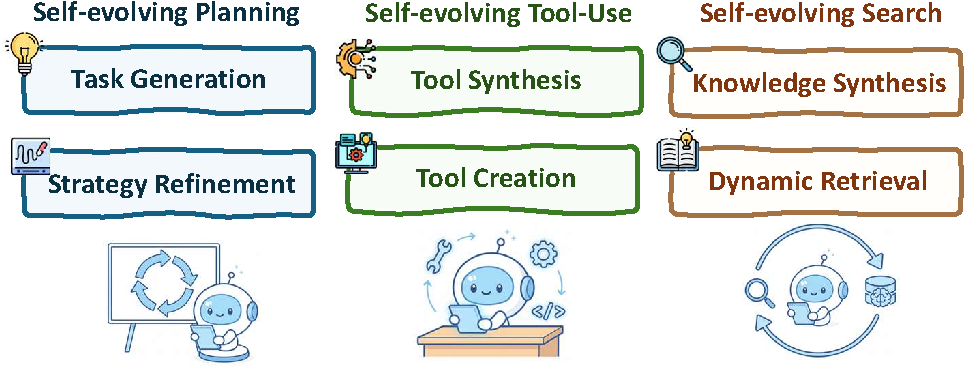
\includegraphics[width=0.8\linewidth]{arxiv/figs/evolve.pdf}
    \caption{An overview of evolving foundational agentic capabilities along three key dimensions: \emph{planning} (task generation and strategy refinement), \emph{tool-use} (tool creation and synthesis), and \emph{search} (dynamic retrieval and knowledge synthesis). These dimensions reflect how agentic systems autonomously enhance their reasoning and problem-solving capacity over time.}
    \label{fig:evolve}
\end{figure}

\subsubsection{Self-evolving Planning}

Recent advances view planning not as a fixed reasoning routine but as an evolving capability. Instead of relying on static datasets or human-designed curricula, agents can autonomously generate tasks, learn from their own feedback, and adapt strategies through iterative interaction with the environment. This enables continuous improvement without external supervision.

A representative direction is self-generated task construction. 
For example, SCA enables agents to alternate between generating problems and solving them, reusing successful trajectories for fine-tuning \cite{zhou2025selfchallenginglanguagemodelagents}. 
Self-rewarding frameworks further allow agents to assess their own outputs, producing high-quality training signals without human labels \cite{simonds2025selfrewardingselfimproving,simonds2025self}. 
Other works directly leverage execution feedback for online adaptation, such as SELF, SCoRe, PAG, TextGrad, and AutoRule, which transform natural-language critiques or traces into training rewards, enabling continual policy refinement \cite{lu2023self,kumar2024training,yuksekgonul2024textgrad,wang2025autorule}.

Beyond internal feedback, agents can also evolve through environment shaping. 
AgentGen constructs adaptive environments to induce curriculum learning \cite{hu2025agentgen}, while Reflexion and AdaPlanner use self-reflective or adaptive strategies to refine plans at runtime \cite{shinn2023reflexion,sun2023adaplanner}. 
Self-Refine iteratively critiques and improves outputs \cite{madaan2023self}, and SICA allows self-modification of code and reasoning tools \cite{robeyns2025self}. 
From an RL perspective, RAGEN and DYSTIL model planning as a Markov Decision Process and optimize strategies with dense feedback \cite{wang2025ragen,wang2025dystil}.

Together, these methods establish a self-improving planning loop, where agents generate their own tasks, shape their environments, and refine strategies, laying the groundwork for autonomous, open-ended planning evolution.

\subsubsection{Self-evolving Tool-use}

\paragraph{Creating and Synthesizing Tools.}
The culmination of in-context reasoning is the emergent capability of agents to autonomously create new tools. This is achieved not through training, but by prompting a frozen LLM to act as a programmer when it encounters a problem that its existing toolset cannot solve.
The LATM framework \cite{cai2024large} uses a powerful model as a one-time "tool maker" and a cheaper, lightweight model as a frequent "tool user," thus amortizing the cost of creation. 
To enable specialization beyond the limits of general-purpose APIs, frameworks like CRAFT \cite{yuan2024craft} and CREATOR \cite{qian-etal-2023-creator} generate custom tools tailored for specific domains. Taking this a step further, ToolMaker \cite{wölflein2025llmagentsmakingagent} can convert entire public code repositories into usable tools, allowing agents to leverage complex, human-written codebases on the fly.



\subsubsection{Self-evolving Search}

Search plays a central role in agentic reasoning, enabling models to retrieve, select, and synthesize relevant knowledge across large and evolving memory spaces. In early systems, search was typically static—built on fixed retrieval heuristics or similarity-based dense retrievers~\cite{lewis2020retrieval,asai2023self,Zhong2023MemoryBankEL,Packer2023MemGPTTL}. These methods augmented prompts with retrieved information but lacked adaptive control over how memory evolves or how search strategies are improved over time.

Recent research increasingly links search and memory in a \textbf{co-evolutionary loop}: agents continuously update their \emph{memory base} during task execution, while dynamically adjusting how search is performed over this evolving knowledge. Agentic memory systems such as MemGPT~\cite{Packer2023MemGPTTL}, MemoryBank~\cite{Zhong2023MemoryBankEL}, and Workflow Memory~\cite{Wang2024AgentWM} already highlight how retrieved information can be synthesized and re-inserted into memory, gradually improving retrieval quality. Dynamic Cheatsheet (DC)~\cite{suzgun2025dynamic} further demonstrates how reusable strategies can be accumulated and leveraged across queries, effectively transforming static search into a \emph{living retrieval substrate} that evolves with agent experience.

\paragraph{Evolving Memory Bases.}  
Unlike static index-based retrieval, self-evolving agents actively refine their memory base through reflection and post-execution updates. Reflexion~\cite{shinn2023reflexion} allows agents to critique their own reasoning traces and store distilled insights, improving future search relevance. Reasoning Bank~\cite{ouyang2025reasoningbank} and context evolution methods~\cite{zhang2025agentic} explicitly restructure memory representations to align retrieval results with evolving problem-solving strategies, effectively making the retrieval target itself adaptive over time.

\paragraph{Dynamic Search and Synthesis.}  
Beyond memory updates, search strategies themselves can evolve through dynamic prioritization and synthesis. Structured memory representations—such as workflows~\cite{Li2024AutoFlowAW,zhang2024aflow,Zeng2023FlowMindAW} and knowledge graphs~\cite{Ouyang2024RepoGraphEA,Edge2024FromLT,chhikara2025mem0,rasmussen2025zep}—provide semantic scaffolding that enables multi-hop and compositional search, supporting richer reasoning over longer horizons. Systems like MemOS~\cite{li2025memos} and Memory-as-Action~\cite{zhang2025memory} take this further by integrating search decisions directly into the reasoning policy, allowing retrieval targets, strategies, and sources to co-adapt as agents accumulate experience.

Overall, self-evolving search transforms retrieval from a static utility into a continuously adapting component of the reasoning loop. By evolving memory bases, dynamically adjusting search strategies, and synthesizing retrieval results into structured knowledge, agents can maintain more relevant, structured, and actionable information over extended time horizons.


